% This work is licensed under the Creative Commons Attribution-NonCommercial 4.0 International License.
% To view a copy of this license, visit http://creativecommons.org/licenses/by-nc/4.0/
% or send a letter to Creative Commons, PO Box 1866, Mountain View, CA 94042, USA.

% !TEX TS-program = xelatex

\documentclass[../Main/chem371-notes.tex]{subfiles}

\setcounter{chapter}{8}
\begin{document}

\chapter{Wave function methods}

In previous chapters we have discussed Hartree--Fock and Kohn--Sham theory.
Now we introduce more advanced wave function methods that introduce correlation effects beyond the level of Hartree--Fock theory in a systematically improvable way.

\mfigure{
\centering{
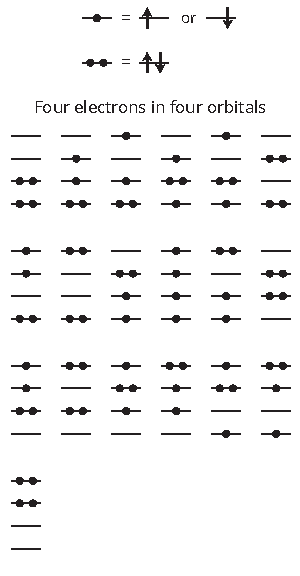
\includegraphics[width=2.00in]{img/fci.pdf}
}
\captionof{figure}{All possible arrangements of four electrons in four orbitals. Each arrangement may correspond to more than one Slater determinant when all possible spins are assigned to the unpaired electrons.}
\label{fig:wfn:fci}
}

All the wave function methods considered here are \emph{post-Hartree--Fock methods}.
They start from the Hartree--Fock wave function and correct it for the missing electron correlation via a correction term ($\Psi_\mathrm{corr}$)
\begin{equation}
\label{eq:wfn:ansatz}
\Psi = \Psi_\mathrm{HF} +  \Psi_\mathrm{corr}
\end{equation}
We will consider three strategies to compute $\Psi_\mathrm{corr}$: 1) the configuration interaction approach, 2) perturbation theory, and 3) coupled cluster methods.
Approaches that are based on Eq.~\eqref{eq:wfn:ansatz} are referred to as \emph{single-reference}, as they are based on the assumption that the HF reference is qualitatively correct.
Therefore, they inherit many of the limitations of HF theory and are mainly applicable near the equilibrium geometry.
Wave function methods specifically designed for low-spin open shells and multideterminantal electronic states exist, but are outside of the scope of this course.


\section{Configuration interaction}



One way to understand how wave function methods work is to consider what the exact solution to the Schr\"{o}dinger equation looks like in the most general case.
We have already encountered the idea of expanding a solution in a fixed basis when we considered how to approximate the orbitals in Hartree--Fock theory.
In this case we wrote an orbital $\varphi_i(\mathbf{r})$ as a linear combination of basis functions $\chi_\mu(\mathbf{r})$ multiplied by the coefficients $C_{\mu}$
\begin{equation}
\varphi(\mathbf{r}) \approx \sum_\mu C_{\mu}\chi_\mu(\mathbf{r})
\end{equation}
The same idea can be used to approximate the wave function of a system with more than one electron.
The main difference is that now the correct way to write this approximation is to \emph{combine all possible Slater determinants} obtained by distributing electrons in a given set of orbitals.
Figure~\ref{fig:wfn:fci} show all possible arrangements of four electrons in four orbitals.
This idea is called \emph{full configuration interaction} (FCI). Expressed mathematically, the CI wave function is a sum of all possible Slater determinants $\Phi_I$ multiplied by the coefficients $C_I$
\begin{equation}
\Psi_\mathrm{CI} = \sum_I^{\text{dets}} C_I \Phi_I
\end{equation}
where the index $I$ enumerates all possible arrangements of the electrons.
In the FCI method, the unknown quantity that has to be determined numerically is the value of the coefficients $C_I$.

It is convenient to take the Hartree--Fock determinant as a reference from which all other determinants are obtained by \emph{exciting electrons}.
The image below shows the FCI wave function expressed in this way.
Determinants obtained by promoting one electron from an occupied to an unoccupied orbital in the HF reference are called \emph{single excitations} or \emph{singly excited determinants} (S).
Similarly, determinants obtained by promoting two electrons are called double excitations (D), those obtained by promoting three electrons triple excitations (T), etc.
For a system containing $N$ electrons, the FCI wave function contains excitations up to at most order $N$.
\begin{center}
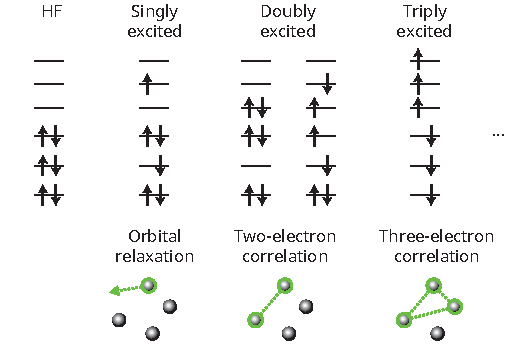
\includegraphics[width=3.5in]{img/fci_expansion_simple.pdf}
\end{center}

\mfigure{
\captionof{table}{Water. Convergence of the energy of truncated CI methods to the FCI limit as a function of the maximum excitation level. These results use the DZ basis and $r_\text{OH}$ = 1.0 \AA{}, $\theta_\text{H-O-H}$ = 104.5 degrees.}
\begin{tabular}{@{} lrr @{}}
\toprule
Method & Determinants & $E_\text{corr}$ (\Eh) \\
\midrule
HF & 1 & $-${\bf76}.005679 \\
CIS & 1 & $-${\bf76}.005679 \\
CISD &  880 & $-${\bf76.1}48415  \\
CISDT & 9808 & $-${\bf76.1}49595 \\
CISDTQ & 61318 & $-${\bf76.156}443 \\
CISDTQP & 225318 & $-${\bf76.156}558 \\
CISDTQPH & 518124 & $-${\bf76.15669}6 \\
CISDTQPH7 & 807052 & $-${\bf 76.15669}8 \\
FCI & 1002708 & $-$76.156699 \\
\bottomrule
\end{tabular}
\label{fig:wfn:fci_water}
}

These different classed of excitations describe different effects.
Single excitations mainly account for orbital relaxation effects, that is, they correct for the way orbitals change in the presence of correlation.
Double excitations are typically the largest contribution to the correlation energy and account for pairwise correlation effects.
Triply and higher-excited determinants are responsible for correlation effects of three or more electrons and usually are a small but play an important role.


\emph{One issue with the FCI expansion is that its size grows exponentially with the number of electrons!}
Whenever a method has exponential scaling, it means that you will quickly run out of computational resources.
To illustrate this point, let's assume that a method that runs in $2^N$ seconds, where $N$ is the number of electrons.
A computation on four electrons would take 16 seconds, one on eight electrons a bit more that four minutes, one on 16 electrons would take 18 hours, and a computation on 32 electrons would take 136 years!
That is why we cannot just apply the FCI method to problem in chemistry.


When the FCI expansion is truncated to a certain excitation level, the corresponding approximation is called \emph{truncated configuration interaction} (CI).
One property of truncated CI methods it that \emph{they are variational}, which means that any truncated CI gives an energy that is greater than or equal to FCI
\begin{equation}
E_\text{Truncated CI} \geq E_\text{FCI}
\end{equation}

Important approximation are CI with singles (CIS) a method used to study excited states, and CI with singles and doubles (CISD).
The convergence of the CI energy as a function of the truncation level for the water molecule is shown in Table~\ref{fig:wfn:fci_water}.
Note that CIS is equivalent to HF (they give the same energy), but as we increase the excitation level the energy systematically converges to the FCI value.
To achieve an error of less than 1 m\Eh it is necessary to go up to quadruple excitations (CISDTQ).

\mfigure{
\centering{
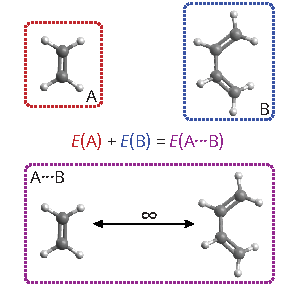
\includegraphics[width=2.00in]{img/size_consistency.pdf}
}
\captionof{figure}{Illustration of the size consistency condition [Eq.~\eqref{eq:wfn:size_consistency}]. The sum of the energy of the molecules A and B must be equal to the energy of A and B at infinite distance.}
\label{fig:wfn:fci}
}

Unfortunately truncated configuration interaction methods are not practically useful methods to study molecules because \emph{they are not size consistent}.
Consider two molecules, A and B.
A computational method is said to be size consistent if the sum of the energy of A and B computed separately is equal to the energy of A and B at infinite separation (A $\cdots$ B)
\begin{equation}
\label{eq:wfn:size_consistency}
E(\text{A}) + E(\text{B}) = E(\text{A} \cdots \text{B}) 
\end{equation}
\emph{Truncated CI methods fail to satisfy this basic requirement}, and that is problematic if we are interested in computing energy changes for reactions that break bonds.

\section{Perturbation theory}

Another systematic path towards the exact solution of the Schr\"{o}dinger equation is perturbation theory.
In perturbation theory we divide the Hamiltonian into an easy part (zeroth-order) that we can solve exactly ($\hat{H}_0$) plus a perturbation ($\hat{V}$).
Then we ask the question: Suppose that we know how to solve the Schr\"{o}dinger equation for the easy part, how does the solution change if we add a tiny bit of the perturbation?
Mathematically, this can be done by introducing a small parameter $\lambda$ defined in the range [0,1], so that the Hamiltonian now depends on $\lambda$
\begin{equation}
\hat{H}_\lambda = \hat{H}_0 + \lambda \hat{V}
\end{equation}
Perturbation theory allows to derive perturbative corrections to the Hartree--Fock energy that are expressed as a series
\begin{equation}
E = E_\text{HF} + E^{(2)} + E^{(3)} + E^{(4)} + \ldots
\end{equation}
where $E^{(2)}$ is the second-order correction, $E^{(3)}$ the third order correction, and so on.

The most widely used form of perturbation theory is the \emph{M{\o}ller--Plesset perturbation method} (MP), defined by the choice $\hat{H}_0 = \hat{f}$, where $\hat{f}$ is the Fock operator that arises in Hartree--Fock theory.
\emph{Contrary to truncated CI, the MP methods are size consistent at every order.}
The \emph{second-order MP energy} (MP2) is defined as
\begin{equation}
E_\text{MP2} = E_\text{HF} + E^{(2)}
\end{equation}
while third-order MP (MP3) contains an extra term
\begin{equation}
E_\text{MP3} = E_\text{HF} + E^{(2)} + E^{(3)}
\end{equation}
MP2 and MP3 are often used to study weak molecular interactions and they are generally not accurate enough to predict thermochemistry.
Some variants of MP methods have been introduced recently, including methods that scale the energy contribution in MP2 and the MP2.5 method, which is defined as the average of the MP2 and MP3 energies
\begin{equation}
E_\text{MP2.5} = \frac{1}{2} (E_\text{MP2} +E_\text{MP3})
\end{equation}


\section{Coupled cluster methods}

One of the most accurate wave function methods are based on coupled cluster (CC) theory.
The CC formalism uses an exponential parameterization of the wave function\mnote{Recall that the Taylor series for the exponential function $e^x$ is
$$
e^x = 1 + x + \frac{1}{2!} x^2 + \frac{1}{3!} x^3 + \frac{1}{4!} x^4 + \ldots
$$
}
\begin{equation}
\Psi_\mathrm{CC} = e^{\hat{T}} \Phi_\text{HF} = \left( 1 + \hat{T} + \frac{1}{2} \hat{T}^2 + \ldots \right) \Phi_\text{HF}
\label{eq:wfn:cc}
\end{equation}
where $\Phi_\text{HF}$ is the Hartree--Fock determinant and $\hat{T}$ is an operator  (cluster operator) that excites electrons from the occupied to the unoccupied Hartree--Fock orbitals.
The cluster operator may be separated according to the number of electrons excited as
\begin{equation}
\hat{T} = \hat{T}_1 + \hat{T}_2 + \hat{T}_3 + \ldots
\end{equation}
where $\hat{T}_1$ applied to $\Phi_\text{HF}$ generates single excitations, $\hat{T}_2$ generates double excitations, etc.
However, as shown in Eq.~\eqref{eq:wfn:cc}, the CC wave function contains powers of the operator $\hat{T}$, for example, terms that are quadratic in $\hat{T}$ lead to several combination of excitation operators
\begin{equation}
\frac{1}{2}\hat{T}^2 = 
\frac{1}{2} (\hat{T}_1 + \hat{T}_2 + \hat{T}_3 + \ldots)^2
= \frac{1}{2} \hat{T}_1^2  + \hat{T}_1\hat{T}_2   +\frac{1}{2} \hat{T}^2_2 + \ldots
\end{equation}
Product terms like $\hat{T}_1^2$ generate double excitations, $ \hat{T}_1\hat{T}_2 $ triple excitations, and so on.
Therefore, even if $\hat{T}$ is truncated, the CC wave function contains excited determinants of all orders.
The exponential structure of CC theory has an important property: \emph{It guarantees that truncated CC methods are size consistent}.

The most widely used CC methods are CC with singles and double (CCSD) defined by the truncation
\begin{equation}
\text{CCSD:}\quad \hat{T} \approx \hat{T}_1 + \hat{T}_2
\end{equation}
and CCSD plus triples ($\hat{T}_3$) treated as a perturbation [CCSD(T)], which is based on the truncation
\begin{iequation}
\text{CCSD(T):}\quad \hat{T} \approx \hat{T}_1 + \hat{T}_2 + \hat{T}_3^{(2)}
\end{iequation}
where $\hat{T}_3^{(2)}$ generates triply excited determinant and is obtained by a perturbative analysis (second order).
The CCSD(T) method is considered to be the \emph{gold standard} of quantum chemistry, because for many applications it can predict \emph{relative} energies with an accuracy equal to or less than 1 \kcal.

More accurate truncation schemes based on CC theory exist like CC with singles, double, and triples (CCSDT), and an analogous perturbative correction [CCSDT(Q)] that includes quadruple excitations.
These methods play an important role in highly accurate predictions of  the thermochemistry and spectroscopy of small molecules in fields like atmospheric chemistry, combustion chemistry, and astrochemistry.

\section{Basis sets and frozen-core treatments for correlated methods}

Contrary to HF and DFT, wave function methods \emph{require larger basis sets}.
For typical wave function computations a triple-$\zeta$ basis (e.g., cc-pVTZ) is the minimum recommended, and quadruple-$\zeta$ basis are necessary to make highly accurate predictions.
There are alternative ways to deal with the more stringent basis set requirement of correlated methods that will be discussed in the next chapter.

Another decision that the user must make when setting up a correlated computation is the treatment of core electrons.
Most properties that chemists are interested in computing are mostly influenced by the electronic structure of the outer most electron shell, the \emph{valence electrons}.
Core electrons---like the pair of electrons occupying the 1s orbital of carbon---are largely unaffected by changes in the valence shell when bonds are formed or electrons are acquired or lost.
This observation justifies simplified treatments of core electrons that are less expensive than all-electron computations.

There are two ways you can approach correlated computations:
\begin{enumerate}
\item The simplest approach is to \emph{freeze the core electrons after they have been optimized at the Hartree--Fock level}.
This approximation neglects the contributions of core electrons to the correlation energy.
\emph{Some basis sets like the cc-pV$X$Z family have been designed specifically to treat only the valence electrons in frozen-core computations}, and should not be used in all-electron computations.

\item The more expensive \emph{all-electron computations} do not freeze the core electrons.
These computations must use basis sets that contain extra p, d, etc. functions to correlate the inner core electrons.
For example, the cc-pCV$X$Z basis sets are designed to treat core correlation in post-Hartree--Fock computations.
These basis sets should only be used in all-electron computations.
\end{enumerate}


\section{Cost and accuracy of wave function methods}

As in the case of DFT, selecting a wave function method that is appropriate for a given computational study requires finding an optimal compromise between cost and accuracy.
Wave function methods have been traditionally more expensive than DFT.
For example, while DFT computation have a computational cost that scales as the fourth power of the number of electrons ($N$), $N^4$, wave function methods scale at least as $N^5$ or higher.

Table~\ref{tab:wfn:comparison} shows a comparison of the cost and properties of the correlated methods considered in this chapter.
note that when combined with density-fitting, some of the methods will result in lower memory cost.
Density fitting will generally increase the speed of computations; however, in most cases it does not change the scaling of the CPU cost as a function of system size.
\begin{table}[htbp]
\centering
\topcaption{Comparison of the properties of various quantum chemistry methods.} % requires the topcapt package
\begin{tabular}{@{} lccc @{}}
\toprule
Method & CPU cost & Memory cost & Size consistent\\
\midrule
Hartree--Fock & $N^4$ &  $N^4$ & Yes \\
DFT & $N^4$ & $N^4$ & Yes \\
CISD & $N^6$ & $N^4$ & No\\
MP2 & $N^4 + N^5$ & $N^4$ & Yes\\
%MP2 (density fitting) & $N^4 + N^5$ & $N^3$ & Yes\\
MP3 & $N^6$ & $N^4$ & Yes \\
CCSD & $N^6$ &$ N^4$ & Yes\\
CCSD(T) & $N^7$ & $N^4$ &Yes\\
%Hartree--Fock (density fitting) & $N^4$ &  $N^3$ & Yes \\
%DFT (local functionals, DF) & $N^3$ & $N^3$ &Yes \\
%DFT (hybrid functionals, DF) & $N^4$ & $N^3$ &Yes \\
\bottomrule
\end{tabular}
\label{tab:wfn:comparison}
\end{table}

\mfigure{
\captionof{table}{Energy of the water molecule computed with various wave function methods and the cc-pVDZ basis set (the 1s-like orbital of oxygen was kept doubly occupied in all computations). All results are based on the experimental geometry of water ($r_\mathrm{OH}$ = 0.958 \AA{}, $\theta_\mathrm{HOH}$ = 104.4776 degrees).}
\begin{tabular}{@{} lcr @{}}
\toprule
Method & Energy & \% of $E_\mathrm{corr}$ \\
\midrule
Hartree--Fock 	&	-76.026761	&	0.00	\\
CISD 	&	-76.229969	&	94.55	 \\
CISDT 	&	-76.232911	&	95.92	 \\
CISDTQ 	&	-76.241369	&	99.85	 \\
MP2 	&	-76.228443	&	93.84	 \\
MP3 	&	-76.235439	&	97.09	 \\
MP4 	&	-76.240679	&	99.53	 \\
CCSD 	&	-76.238010	&	98.29	 \\
CCSD(T) 	&	-76.241048	&	99.70	 \\
FCI (= exact) 	&	-76.241683	&	100.00	 \\
%Hartree--Fock & -76.026761 \\
%CISD & -76.229969 & \\
%CISDT & -76.232911 & \\
%CISDTQ & -76.241369 & \\
%MP2 & -76.228443 & \\
%MP3 & -76.235439 & \\
%MP4 & -76.240679 & \\
%CCSD & -76.238010 & \\
%CCSD(T) & -76.241048 & \\
%FCI (= exact) & -76.241683 & \\
\bottomrule
\end{tabular}
\label{tab:wfn:Ecorr}
}


It is interesting to compare the absolute accuracy of different correlated methods.
Table~\ref{tab:wfn:Ecorr} reports the total energy and the percentage of the correlation energy recovered by each method for the water molecule using a cc-pVDZ basis.
For this molecule, the correlation energy is -0.21492 \Eh (about 135 \kcal).
All methods recover more than 90\% of the correlation energy, but there are significant differences in the relative performance.
Among the methods that include up to doubles, CCSD recovers 98.3 \% vs. 94.6 \% for CISD.
In CI adding triples only leads to recovering 95.9 \% of the correlation energy.
Instead, CCSD(T) already recovers 99.70 \% of $E_\mathrm{corr}$.
Only when full quadruples are added in CI, the energy is comparable to that of CCSD(T).
Why is the CCSD method so accurate? As the CISDTQ computation show, quadruple excitations are the largest contribution to $E_\mathrm{corr}$ after doubles (singles and triples play a minor role).
In CCSD the wave function contains quadruple excitations from the quadratic terms of the form $\frac{1}{2} \hat{T}_2^2$ and these are already a good approximation of the quadruples.
The MP series also shows quick convergence to the FCI limit.
However, \emph{there are instances when the MP series does not converge}. Therefore, CC methods are generally preferred to MP perturbation theory.

Many implementations of wave function methods can now employ density-fitted two-electron integrals.
This greatly reduces the storage cost of these methods.
For example, density-fitted MP2 has a cost that is negligible compared to Hartree--Fock theory.
Nevertheless, in recent years there have been major efforts dedicated to developing \emph{local} correlation methods that reduce the cost of conventional wave function methods by exploiting the local nature of (dynamical) electron correlation.
For large systems, \emph{linear scaling methods} aim to achieve a scaling linear in $N$.
Linear-scaling versions of many of the methods discussed in this chapter have been developed and are implemented in various codes (e.g., Orca, Molpro).






\end{document}